\documentclass[10pt,twocolumn,letterpaper]{article}
\usepackage[review]{cvpr}
\usepackage{graphicx,booktabs,multirow,amsmath,amssymb,xcolor}
\usepackage[pagebackref,breaklinks,colorlinks,citecolor=blue,linkcolor=blue,urlcolor=blue]{hyperref}
\def\confName{CVPR}\def\confYear{2027}\def\paperID{****}
\newcommand{\Tfull}{\textsc{T-full}}\newcommand{\ARdiff}{\textsc{AR-diff}}
\newcommand{\Sbi}{\textsc{S-bi}}\newcommand{\Scausal}{\textsc{S-causal}}
\newcommand{\ci}[2]{[#1,\,#2]}

\title{Mode-Seeking Meets Autoregression:\\A Training-Free Factorial Diagnosis of Diversity Collapse in Few-Step Video Generators}
\author{Anonymous CVPR submission}

\begin{document}
\maketitle

\begin{abstract}
Few-step distillation makes video diffusion models fast, and a growing literature reports that it also makes them worse: motion collapses, diversity shrinks, colours saturate. Every such report comes from a paper proposing a fix, each with its own metric, so the losses cannot be compared, and none of them separates the effects of \emph{fewer steps}, \emph{rewritten weights} and \emph{causal (autoregressive) architecture}, which real streaming students combine. We disentangle them with a $2{\times}2$ factorial design built entirely from public checkpoints of one model family (Wan2.1-1.3B): \{bidirectional, causal\}$\times$\{50-step, few-step distilled\}, replicated in two independent labs, at three teacher guidance scales, across 20 student recipes and 5{,}405 videos, with a five-axis, non-aggregated evaluation protocol calibrated against blind pairwise human judgements. We find that the loss of cross-seed diversity is an \emph{interaction}: causalisation alone and bidirectional DMD alone cost little, while their combination collapses diversity (interaction $-0.063$, 95\%\,CI $\ci{-0.092}{-0.036}$, sign-stable across guidance scales and feature spaces). The interaction is driven by the distillation objective, not the architecture: it vanishes under consistency distillation and halves under adversarial training, and more than half of it is already incurred at the ODE-regression initialisation stage that precedes DMD. It is fully present in the first generated chunk and then merely propagated by the KV cache; chunk size does not modulate it. Taxes on other axes have opposite signs---causalisation costs temporal coherence, which distillation refunds---so no scalar can rank these models. Finally, four frame-level image-quality metrics rank distilled students \emph{above} their teacher while humans rank the teacher far above all students: the ``quality improves after distillation'' numbers in the literature are a metric artefact. Corpus, per-video metrics and scripts are released.
\end{abstract}

\section{Introduction}
Streaming and interactive video generation runs on few-step, causal students distilled from bidirectional multi-step teachers: CausVid~\cite{causvid}, Self-Forcing~\cite{selfforcing}, Causal Forcing~\cite{causalforcing}, Causal-rCM~\cite{causalrcm}. The cost of this speed-up is visible to anyone who samples the same prompt with different seeds---the student returns the same shot again and again (Fig.~\ref{fig:teaser})---and it has been documented repeatedly: dynamic degree dropping from $0.80$ to $0.00$~\cite{dynaforcing}, diversity collapse~\cite{uncertaintydmd,dataforcing}, temporal collapse and oversaturation~\cite{avd}. Each of these papers proposes a remedy and reports the degradation that its remedy repairs, with its own metric and its own baseline. Three things are therefore still unknown. (i)~\emph{Whose fault is it?} A causal DMD student differs from its teacher in three ways at once---fewer sampling steps, distilled weights, and a causal architecture with a KV cache---and no comparison in the literature includes the cell that isolates the third: a causal model that is \emph{not} distilled. (ii)~\emph{Which recipe?} DMD, SiD, consistency, adversarial and ODE-regression objectives are all in use, with and without self-rollout training, at different chunk sizes; their losses have never been measured under one protocol. (iii)~\emph{Which metric?} Distillation papers routinely report that imaging-quality scores go \emph{up} while motion goes down~\cite{dynaforcing}; whether that reflects perception has not been tested.

We answer all three without training anything. The Wan2.1-1.3B family is unique in that public checkpoints exist for every cell of a $2{\times}2$ factorial design---bidirectional or causal architecture, 50-step or few-step distilled sampling---from two independent labs (CausVid/Causal-Forcing and NVIDIA Causal-rCM), together with twelve further students that vary the objective (DMD, SiD, GAN, discrete/continuous consistency), the training stage (ODE-regression init, consistency init, DMD refinement), the exposure regime (teacher forcing vs.\ self-rollout) and the chunk size (1 or 3 latent frames). We generate every configuration on the same 30 prompts and the same initial noise, measure five capability axes with one primary metric each (mode coverage, cross-seed diversity, object motion, prompt adherence, temporal coherence), never aggregate across axes, and calibrate the axes that matter against 90 blind pairwise human judgements.

\paragraph{Findings.} (1)~\textbf{The diversity tax is an interaction.} Causalising the teacher costs almost no diversity ($-0.006$), bidirectional DMD costs little ($-0.017$), but the two together cost $-0.086$; the interaction term is $-0.063$ $\ci{-0.092}{-0.036}$ and keeps its sign when the teacher's guidance scale is changed from 3 to 7.5 and when the feature space is changed (\S\ref{sec:interaction}). (2)~\textbf{The interaction belongs to the objective, not the architecture.} With a consistency objective the same causal architecture shows \emph{no} negative interaction (and a positive one on coverage, $+0.48$ $\ci{0.28}{0.69}$); adding self-rollout DMD on top of the consistency initialisation brings it back ($-0.035$ $\ci{-0.063}{-0.008}$); SiD behaves like DMD; GAN collapses about half as much (\S\ref{sec:recipe}). (3)~\textbf{Most of the loss precedes DMD.} Along the public training ladders, the ODE-regression initialisation already removes more than half of the diversity that the final DMD student lacks; consistency initialisation does not (\S\ref{sec:stage}). (4)~\textbf{It happens in the first chunk.} Per-frame diversity of causal DMD students is fully depressed at frame~0 and flat afterwards; undistilled causal models instead \emph{gain} diversity along the video through autoregressive drift, which is where their temporal tax comes from. Chunk size (1 vs.\ 3 latent frames) does not modulate the collapse---a mechanism prediction we made and that failed (\S\ref{sec:stage}). (5)~\textbf{Taxes have opposite signs across axes.} Causalisation costs temporal coherence and distillation refunds it (positive interaction in every configuration); prompt adherence is untaxed; camera motion is taxed two to three times more than object motion; oversaturation appears with causal fine-tuning, not with DMD (\S\ref{sec:axes}). (6)~\textbf{Frame-level quality metrics are inverted on distilled video.} MUSIQ, CLIP-IQA, MANIQA and TOPIQ all rank DMD students above the teacher; a human ranks the teacher above every student with a 35.5/36 win rate, and two of the metrics agree with the human significantly \emph{below} chance (\S\ref{sec:iqa}).

\section{Related work}
\paragraph{Few-step and causal distillation.} DMD~\cite{dmd,dmd2} matches the student's output distribution to the teacher's score through a fake-score network and is the workhorse of video distillation (FastWan~\cite{fastwan}, CausVid~\cite{causvid}). CausVid converts the bidirectional Wan2.1 into a block-causal autoregressive model with a KV cache; Self-Forcing~\cite{selfforcing} trains on the student's own rollouts to remove exposure bias; Causal Forcing~\cite{causalforcing} adds a teacher-forced causal diffusion stage and an asymmetric DMD; Causal-rCM~\cite{causalrcm,rcm} replaces the initialisation with teacher-forced consistency distillation before self-forcing DMD. SiD~\cite{sid} and adversarial variants are released alongside Self-Forcing. We use all of these as they were published; we train nothing.

\paragraph{Reported degradations.} DynaForcing~\cite{dynaforcing} documents the dynamic-degree collapse of Self-Forcing under extended training; Adaptive Video Distillation~\cite{avd} attributes oversaturation and temporal collapse to distribution-matching losses; Data-Forcing~\cite{dataforcing} and Uncertainty DMD~\cite{uncertaintydmd} attribute diversity collapse to DMD's mode seeking, the latter proposing that a collapsed first chunk is propagated by the deterministic cache; CoDMD~\cite{codmd} shows the sign of the degradation flips with model scale. All are method papers. We confirm the mechanism of~\cite{uncertaintydmd} with a factorial design that isolates it, and add that it is objective-specific, mostly incurred before DMD, and invisible to standard quality metrics.

\paragraph{Evaluation.} VBench~\cite{vbench} aggregates sixteen dimensions; its dynamic-degree and smoothness dimensions are anti-correlated by construction, which we quantify. Precision/recall in feature space~\cite{prdc,kynk} separate fidelity from coverage; we use them on VideoMAE~\cite{videomae} and DINOv2~\cite{dinov2} features. No-reference IQA (MUSIQ~\cite{musiq}, CLIP-IQA~\cite{clipiqa}, MANIQA~\cite{maniqa}, TOPIQ~\cite{topiq}) is used as ``imaging quality'' in video benchmarks; we test it against human judgement on distilled video.

\section{Protocol}\label{sec:protocol}
\paragraph{Configurations.} All models share the Wan2.1-T2V-1.3B backbone, the same VAE, the same cached UMT5-XXL prompt embeddings, the same attention kernel and the same generation setting (81 frames, $480{\times}832$, 16\,fps, identical initial noise per seed). Table~\ref{tab:cells} lists the cells. The teacher (\Tfull) uses Wan's default sampler (UniPC, 50 steps, shift~5, CFG~5). The undistilled causal cells (\ARdiff) are the teacher-forced causal diffusion checkpoints released by Causal-Forcing (chunk of 3 latent frames) and by Causal-rCM (\texttt{TF\_Diffusion}), sampled with the same UniPC/CFG setting through their KV-cache pipeline. Bidirectional distilled cells are CausVid's bidirectional DMD checkpoint and NVIDIA's rCM; causal distilled cells are CausVid's autoregressive DMD, Self-Forcing (DMD, SiD, SiD-v2, GAN), Causal-Forcing (DMD, consistency, ODE-init, frame-wise), and Causal-rCM (TF-dCM, TF-dCM$+$SF-DMD, both at chunk 3 and chunk 1). Each student is sampled with its authors' own schedule. FastWan~\cite{fastwan} is included as a secondary bidirectional DMD cell (it was trained with sparse attention; we run it densely). Two sets of controls address confounds: \textsc{T-few} (the teacher at 4 steps) isolates \emph{fewer steps}; \textsc{T-cfg}$\{1,3,7.5\}$ and \ARdiff-cfg$\{3,7.5\}$ trace the guidance scale, because distilled students absorb guidance and DMD targets the teacher at a real-score guidance of 3--3.5.

\begin{table*}[t]\centering\small
\caption{Cells of the factorial design (all Wan2.1-1.3B, 81 frames, $480{\times}832$). TF = teacher-forced context during training, SR = self-rollout. $n$ = videos with 8 seeds unless noted.}\label{tab:cells}
\begin{tabular}{@{}llll@{}}\toprule
cell & architecture & objective / stage & source \\\midrule
\Tfull & bidirectional, 50 steps & --- & Wan2.1 \\
\ARdiff & causal, 50 steps & TF diffusion & Causal-Forcing \\
\ARdiff-rcm & causal, 50 steps & TF diffusion & Causal-rCM \\
\Sbi-causvid & bidirectional, 3 steps & DMD & CausVid \\
\Sbi-rcm & bidirectional, 4 steps & consistency (rCM) & NVIDIA \\
\Scausal-causvid & causal, 3 steps & DMD, TF & CausVid \\
S-sf / -sid / -sid2 / -gan & causal, 4 steps & DMD / SiD / GAN, SR & Self-Forcing \\
S-cf / -cd / -ode / -fw & causal, 4 steps & DMD(SR) / CM / ODE-init / chunk\,1 & Causal-Forcing \\
S-rcm-tfdcm (-fw) & causal, 4 steps & consistency, TF (chunk 1) & Causal-rCM \\
S-rcm-sfdmd (-fw) & causal, 4 steps & CM init $+$ SR-DMD (chunk 1) & Causal-rCM \\
S-causvid-ode & causal, 3 steps & ODE-regression init & CausVid \\
T-few, T-cfg$c$, AR-diff-cfg$c$ & controls & 4 steps; CFG $c$ ($n{=}4$ seeds) & --- \\\bottomrule
\end{tabular}
\end{table*}

\paragraph{Prompts and seeds.} 30 prompts fixed before any generation: 15 VBench sentences covering static, slow and dynamic content, and 15 written to hit the regimes reported as distillation-sensitive (fast motion, multi-object interaction, rare compositions, object-count conservation, physical events). Eight seeds per prompt; seeds map to identical initial latent noise in every cell, so all cell comparisons are paired.

\paragraph{Five axes, one primary metric each.} \textbf{A1 coverage}: $k$-NN manifold recall of the teacher's samples by the student's ($k{=}3$)~\cite{kynk}, pooled over prompts, VideoMAE-base features (DINOv2-L frame features as a second space); precision is always reported alongside so that ``garbage is diverse'' cannot pass. \textbf{A2 diversity}: mean pairwise cosine distance among the 8 seeds of a prompt in the same feature spaces. \textbf{A3 motion}: RAFT flow decomposed by robust affine fitting into a global (camera) and a residual (object) field; the residual magnitude is primary, the global one reported. \textbf{A4 adherence}: BLIP-2 yes/no VQA on three pre-registered questions per prompt (CLIP-T alongside). \textbf{A5 temporal coherence}: RAFT backward-warp error (lower is better). We never combine axes into a score.

\paragraph{Statistics.} Every contrast is paired over the 30 prompts (the same seeds and noise appear in every cell): prompt-level bootstrap CIs for A2--A5, leave-one-prompt-out jackknife for the set-level A1. The $2{\times}2$ interaction is $I=(D_{\text{causal}}-D_{\text{bi}})_{\text{distilled}}-(D_{\text{causal}}-D_{\text{bi}})_{\text{50-step}}$ computed per prompt and bootstrapped. Rank structure across cells is summarised by the eigenvalue spectrum of the axis-correlation matrix and by counting significant rank reversals (two cells ordered oppositely on two axes, both $|z|>1.96$).

\paragraph{Human calibration.} One rater (an author; a limitation) judged 90 blind pairwise comparisons: for a prompt, four seeds of cell $A$ vs.\ four seeds of cell $B$, autoplaying side by side, answering which side is more diverse across seeds, which has more natural motion, and which has better image quality. Six cells, a balanced round-robin design (each of the 15 pairs six times, left/right randomised); Bradley--Terry scores with ties as half wins.

\section{Results}
\begin{figure}[t]\centering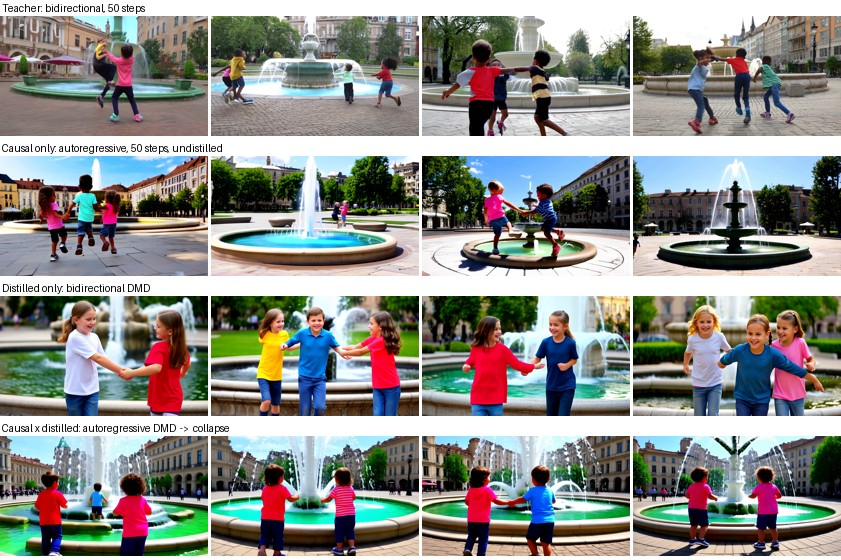
\includegraphics[width=0.98\linewidth]{figures/fig_teaser.jpg}
\caption{One prompt (``three children chasing each other around a fountain''), four seeds, middle frame. Neither causalising the teacher (row~2) nor bidirectional DMD (row~3) destroys cross-seed variety; the causal DMD student (row~4) returns the same composition for every seed.}\label{fig:teaser}\end{figure}

\begin{figure*}[t]\centering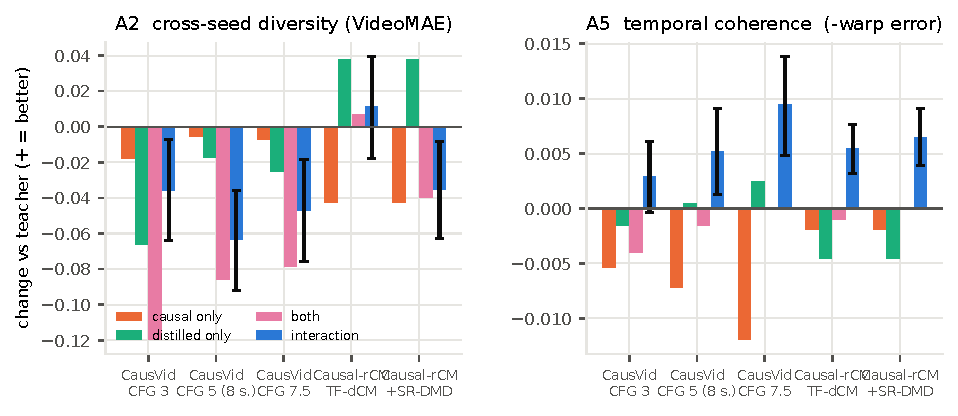
\includegraphics[width=\textwidth]{figures/fig_interaction.pdf}
\caption{$2{\times}2$ main effects and interaction for diversity (left) and temporal coherence (right), each bar the change from the teacher, error bars the 95\% prompt-paired bootstrap CI of the interaction. Left three groups: CausVid cells with the teacher at CFG 3/5/7.5. Right two: the NVIDIA Causal-rCM cells with a consistency-distilled causal student (no interaction) and the same student after self-rollout DMD (interaction returns). Temporal coherence shows the opposite sign everywhere: causalisation costs it, distillation refunds it.}\label{fig:interaction}\end{figure*}

\subsection{The diversity tax is an interaction}\label{sec:interaction}
Table~\ref{tab:main} gives the primary metrics for the key cells; Fig.~\ref{fig:interaction} the factorial decomposition. Causalising the teacher without distilling it leaves cross-seed diversity essentially intact ($0.161\to0.155$) and costs a quarter of the coverage; bidirectional DMD costs a little diversity ($\to0.144$) and half the coverage; the causal DMD student loses more than either sum: diversity $0.075$, recall $0.03$. The prompt-paired interaction is $-0.063$ $\ci{-0.092}{-0.036}$ ($P(I\ge0)<10^{-4}$), larger in magnitude than both main effects together. It replicates in DINOv2 feature space ($-0.065$ $\ci{-0.115}{-0.017}$) and is sign-stable when the two 50-step cells are re-sampled at CFG~3 ($-0.036$ $\ci{-0.064}{-0.007}$) or CFG~7.5 ($-0.047$ $\ci{-0.076}{-0.018}$), which brackets the guidance the students actually absorbed. The interaction is visible to the eye (Fig.~\ref{fig:teaser}) and to the rater: the causal DMD student won 3.5 of 25 diversity comparisons.

Two alternative explanations are excluded. \emph{Fewer steps}: the 4-step teacher is worse than every student on coverage (recall $0.35$, precision $0.50$) and adherence, but \emph{more} diverse than the teacher (0.169)---few-step sampling produces blurry, varied garbage, not a collapsed mode; distillation relative to it is a refund. \emph{High effective guidance}: the teacher's diversity falls from $0.198$ (CFG 3) to $0.161$ (5) and saturates at $0.157$ (7.5); bidirectional DMD students (0.144--0.154) sit near the teacher's high-guidance end, but causal DMD students (0.075--0.134) lie below any guidance setting of the teacher (Fig.~\ref{fig:pareto}, right).

\begin{table*}[t]\centering\footnotesize\setlength{\tabcolsep}{4pt}
\caption{Primary metrics for the key cells (30 prompts $\times$ 8 seeds). Recall/precision are $k$-NN manifold metrics against the teacher in VideoMAE space; diversity is the pairwise cosine distance over seeds; motion in px/frame; VQA is BLIP-2 $P(\text{yes})$; warp error lower is better; colourfulness~\cite{hasler}; MUSIQ is VBench's imaging-quality metric; human BT scores from \S\ref{sec:iqa}.}\label{tab:main}
\begin{tabular}{@{}lccccccccccc@{}}\toprule
 & \multicolumn{2}{c}{A1 coverage} & \multicolumn{2}{c}{A2 diversity} & \multicolumn{2}{c}{A3 motion} & A4 & A5 & & & human \\
cell & recall & prec. & VideoMAE & DINOv2 & object & camera & VQA & warp & colour & MUSIQ & div / qual \\\midrule
\Tfull & 0.97 & 0.88 & 0.161 & 0.350 & 3.69 & 5.71 & 0.678 & 0.016 & 51 & 68.2 & $+1.1$ / $+3.7$ \\
\ARdiff (Causal-Forcing) & 0.61 & 0.62 & 0.155 & 0.303 & 3.44 & 4.83 & 0.672 & 0.023 & 77 & 65.8 & $+0.4$ / $-0.6$ \\
\ARdiff-rcm (NVIDIA) & 0.39 & 0.75 & 0.119 & 0.268 & 3.02 & 4.10 & 0.666 & 0.018 & 87 & 67.5 & --- \\
\Sbi-causvid & 0.33 & 0.40 & 0.144 & 0.232 & 3.15 & 3.36 & 0.673 & 0.016 & 77 & 73.0 & $-0.6$ / $-0.5$ \\
\Sbi-rcm (consistency) & 0.69 & 0.41 & 0.199 & 0.311 & 3.07 & 3.53 & 0.682 & 0.021 & 60 & 69.1 & --- \\
\Scausal-causvid (DMD, TF) & \textbf{0.03} & 0.56 & \textbf{0.075} & \textbf{0.120} & 2.56 & 2.55 & 0.678 & 0.018 & 80 & \textbf{73.8} & $\mathbf{-1.8}$ / $-1.6$ \\
S-sf (DMD, SR) & 0.32 & 0.74 & 0.118 & 0.271 & 3.24 & 3.47 & 0.682 & 0.019 & 62 & 71.6 & $+0.3$ / $+0.7$ \\
S-sf-gan & 0.47 & 0.54 & 0.151 & 0.317 & 2.39 & 2.74 & 0.684 & 0.017 & 65 & 71.1 & --- \\
S-cf-cd (consistency) & 0.75 & 0.53 & 0.192 & 0.464 & 1.35 & 1.81 & 0.679 & \textbf{0.011} & 54 & 63.8 & --- \\
S-rcm-tfdcm (consistency) & 0.60 & 0.56 & 0.168 & 0.394 & 2.34 & 3.10 & 0.676 & 0.017 & 70 & 65.1 & $+0.7$ / $-1.8$ \\
S-rcm-sfdmd (CM $+$ SR-DMD) & 0.21 & 0.57 & 0.121 & 0.246 & 2.07 & 1.92 & 0.682 & 0.016 & 72 & 71.9 & --- \\
T-few (teacher, 4 steps) & 0.35 & 0.50 & 0.169 & --- & 4.00 & 8.05 & 0.650 & 0.018 & 49 & 42.5 & --- \\\bottomrule
\end{tabular}
\end{table*}

\subsection{The interaction belongs to the objective}\label{sec:recipe}
Replacing the causal DMD cell by other students keeps the two 50-step cells fixed and changes only the objective (Fig.~\ref{fig:recipes}, Table~\ref{tab:main}). With NVIDIA's teacher-forced \emph{consistency}-distilled causal student the interaction on diversity is $+0.011$ $\ci{-0.018}{+0.040}$, on DINOv2 diversity $+0.166$ $\ci{0.116}{0.220}$ and on coverage $+0.48$ $\ci{0.28}{0.69}$: a mode-covering objective on a causal architecture \emph{recovers} coverage rather than losing it. Refining that same student with self-rollout DMD brings the negative interaction back ($-0.035$ $\ci{-0.063}{-0.008}$). Within the Self-Forcing family, where architecture, data and self-rollout training are held fixed, SiD and SiD-v2 are indistinguishable from DMD on diversity (differences $\le0.01$, CIs cross zero) while the adversarial student is significantly more diverse ($+0.034$ $\ci{0.022}{0.047}$, recall $0.47$ vs.\ $0.32$). The two consistency cells from two labs and the adversarial cell also show what those objectives pay instead: object motion of $1.35$--$2.4$\,px/frame against the teacher's $3.7$, and precision of $0.53$--$0.56$. Self-rollout training, the fix proposed by Self-Forcing, halves the interaction ($-0.063\to-0.035$) but does not remove it; its entire benefit over CausVid is in the interaction term---the main effects are unchanged.

\begin{figure}[t]\centering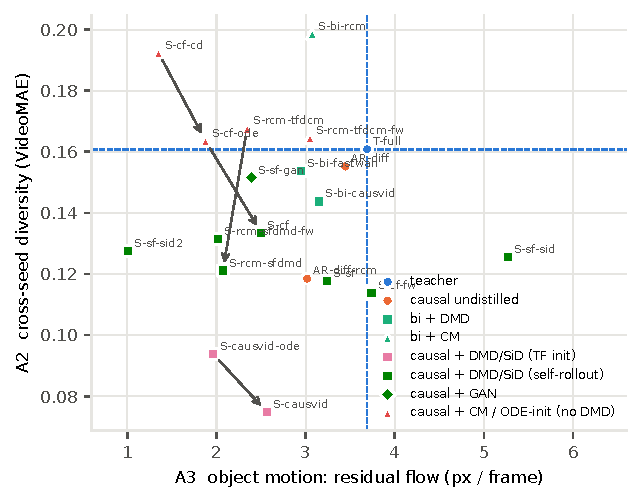
\includegraphics[width=\linewidth]{figures/fig_recipes.pdf}
\caption{Every cell in the diversity--motion plane. Dashed lines: the teacher. Arrows follow public training ladders (consistency $\to$ ODE-init $\to$ DMD in Causal-Forcing; ODE-init $\to$ DMD in CausVid; consistency $\to$ self-rollout DMD in Causal-rCM): each step trades diversity for motion. Mode-seeking objectives (squares) sit low, mode-covering and adversarial ones (triangles, diamond) high.}\label{fig:recipes}\end{figure}

\subsection{Where and when the loss is incurred}\label{sec:stage}
\paragraph{Stage.} The public ladders let us place the loss in training time. In CausVid, the ODE-regression initialisation---a causal model regressed onto teacher ODE trajectories, no DMD yet---already has diversity $0.094$ against the teacher's $0.161$; DMD refinement takes it to $0.075$ (paired difference $+0.019$ $\ci{0.006}{0.033}$; DINOv2 $+0.149$ $\ci{0.109}{0.186}$). More than half of the final deficit is incurred before any distribution matching: regressing each noise onto a single teacher endpoint is itself mode-seeking. In Causal-Forcing the ladder is monotone in both directions---consistency $0.192$ $\to$ ODE-init $0.164$ $\to$ DMD $0.133$ (each step's CI excludes zero) while object motion rises $1.35\to1.88\to2.50$\,px/frame. ODE-init is also the worst cell on every fidelity axis (recall $0.01$, MUSIQ $42$), so DMD's role in these pipelines is to buy fidelity back with the diversity that remains.

\paragraph{Frame.} Fig.~\ref{fig:perframe} plots cross-seed diversity per frame. For causal DMD students the deficit is complete at frame~0 (S-causvid $0.146$ vs.\ teacher $0.403$) and the curve is flat: the KV cache propagates a collapsed first chunk and does not deepen it, consistent with the mechanism hypothesised by~\cite{uncertaintydmd}. Undistilled causal models show the opposite profile---diversity \emph{grows} along the video ($0.345\to0.441$) as autoregressive drift accumulates---which is precisely the temporal tax they pay (\S\ref{sec:axes}).

\paragraph{Chunk size---a failed prediction.} If a mode-seeking objective collapses the first chunk because the chunk has few degrees of freedom, smaller chunks should collapse more. They do not: moving from 3-frame to 1-frame chunks makes Causal-Forcing's DMD student less diverse ($-0.020$ $\ci{-0.034}{-0.007}$) but NVIDIA's self-rollout DMD student \emph{more} diverse (DINOv2 $+0.043$ $\ci{0.012}{0.073}$), and leaves the consistency student unchanged. The first-chunk localisation stands; the degrees-of-freedom explanation does not.

\begin{figure}[t]\centering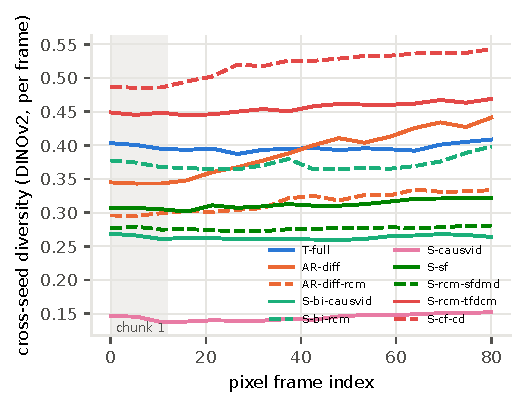
\includegraphics[width=\linewidth]{figures/fig_perframe.pdf}
\caption{Per-frame cross-seed diversity (DINOv2, 8 seeds $\times$ 30 prompts). Distilled causal students are depressed from the first frame and flat; undistilled causal models drift apart along the video.}\label{fig:perframe}\end{figure}

\subsection{Opposite signs on the other axes}\label{sec:axes}
\paragraph{Temporal coherence is refunded.} Causalisation raises warp error ($0.016\to0.023$; subject consistency $0.954\to0.923$; visibly, late chunks blur and drift), distillation lowers it, and the $2{\times}2$ interaction is positive in every configuration we ran---CausVid cells at CFG 3/5/7.5 ($+0.003$, $+0.005$, $+0.010$), NVIDIA cells with either student ($+0.005$, $+0.007$)---with the CI excluding zero in four of five (CFG~3 is borderline). Few-step students do not drift because their rollouts are short and, in the self-rollout recipes, trained on.
\paragraph{Camera motion is taxed more than object motion.} Every student loses 40--70\% of the global (camera) flow ($5.7\to1.8$--$3.5$\,px/frame) but only 10--45\% of the residual (object) flow; the decomposition is needed to see that ``motion collapse'' is largely the loss of camera moves.
\paragraph{Adherence is untaxed.} BLIP-2 VQA on pre-registered attribute questions is $0.66$--$0.69$ for every cell including the teacher; CLIP-T likewise. Mode seeking keeps each sample on-prompt; what is lost is the set, not the sample.
\paragraph{Oversaturation is not a DMD signature.} Colourfulness rises with guidance in the teacher (CFG 3: 36, CFG 5: 50) and is $63$--$79$ in the causal 50-step cells at matched guidance---before any distillation. DMD students (63--80) merely inherit it.
\paragraph{Consequence.} Across 13 non-reference cells the second eigenvalue of the axis-correlation matrix carries 32\% of the variance (28\% among students) and 59 cell pairs (14 among students) are ordered oppositely on two axes with both differences significant. No scalar summary---VBench's total included---can rank these models without hiding a tax.

\begin{figure*}[t]\centering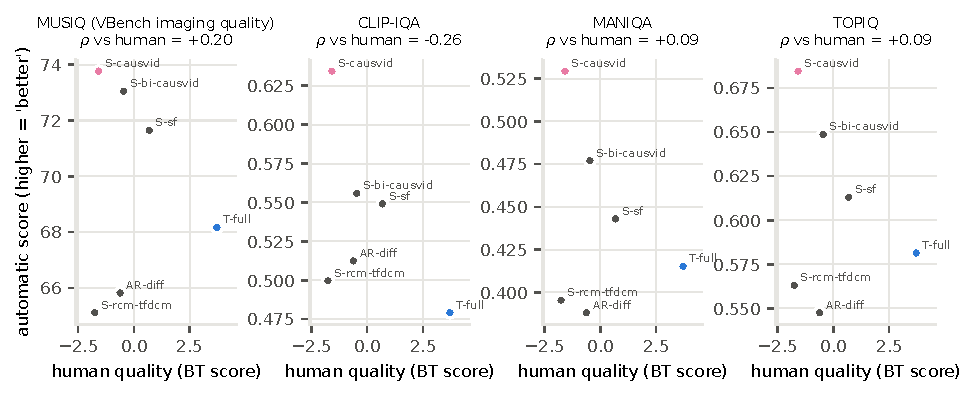
\includegraphics[width=\textwidth]{figures/fig_iqa_human.pdf}
\caption{Four no-reference image-quality metrics against the blind human quality score (Bradley--Terry, 90 pairwise comparisons). All four place the causal DMD student (pink) above the teacher (blue); the human places the teacher above every student.}\label{fig:iqa}\end{figure*}

\subsection{Quality metrics are inverted on distilled video}\label{sec:iqa}
The rater's diversity judgements track our metrics (cell-level Spearman $0.94$ with DINOv2 diversity, $0.89$ with VideoMAE diversity and with recall; per-comparison agreement 83\%, binomial $p<10^{-5}$), and motion judgements track object flow at the cell level ($\rho=0.83$). Quality is different. The rater preferred the teacher in 35.5 of 36 comparisons (BT $+3.7$, next best $+0.7$), yet MUSIQ, CLIP-IQA, MANIQA and TOPIQ---computed on eight frames per video over the whole corpus---all rank the causal DMD student \emph{first} and the teacher fourth or lower (Fig.~\ref{fig:iqa}). Per-comparison agreement with the human is 47\%, 36\%, 39\% and 36\%; for CLIP-IQA and TOPIQ this is significantly below chance ($p=0.027$). The metrics do detect blur (the 4-step teacher and the ODE-init cells score 42) but reward the over-sharpened, over-saturated look of distilled samples. The widely reported observation that imaging quality \emph{improves} after distillation while dynamics collapse~\cite{dynaforcing} is, on this evidence, an artefact of the metric.

\begin{figure*}[t]\centering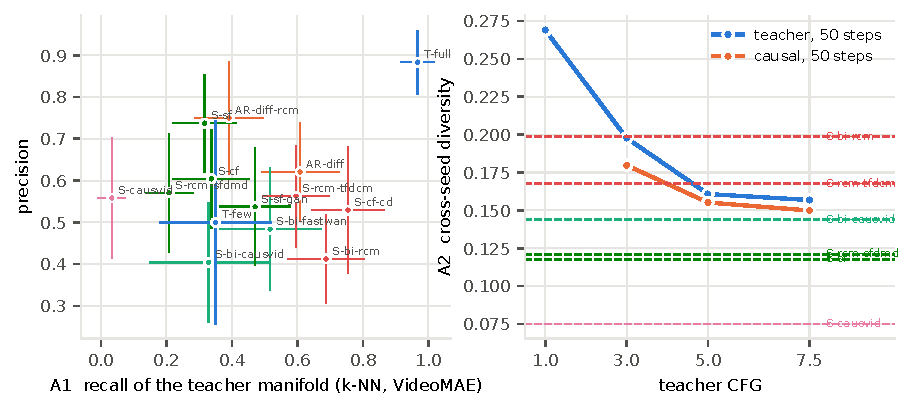
\includegraphics[width=\textwidth]{figures/fig_pareto.pdf}
\caption{Left: coverage against fidelity (jackknife 95\% CIs). Right: the teacher's and the undistilled causal model's diversity as a function of guidance, with students as horizontal lines; causal DMD students lie below any guidance setting.}\label{fig:pareto}\end{figure*}

\section{Discussion}
\paragraph{For practitioners.} Choosing a streaming student is a choice of objective before architecture. Consistency-distilled causal students keep the teacher's coverage and diversity and pay in motion and sharpness; DMD and SiD students keep prompt adherence and per-sample fidelity and pay in coverage; adversarial training sits between. Self-rollout training and consistency initialisation each recover a quantified part of the collapse, and the ODE-regression initialisation still used by several pipelines is where most of it starts. Imaging-quality scores should not be used to compare a distilled model with its teacher.
\paragraph{For evaluation.} The protocol is training-free and needs only public checkpoints: sample every cell on the same noise, report one primary metric per axis with paired CIs, add the undistilled causal cell whenever a causal student is evaluated, trace the teacher's guidance curve, and calibrate any automatic quality axis against humans before reporting it.

\section{Limitations}
All results are on one family, Wan2.1-1.3B, the only one for which every factorial cell is public; the 14B and Wan2.2 counterparts do not fit our single 32\,GB GPU. The undistilled causal cells come from two labs whose checkpoints differ in data and fine-tuning, and their main effects differ (Causal-Forcing's model keeps diversity and drifts; NVIDIA's loses diversity and does not); we therefore report both and draw conclusions only from contrasts that replicate. Prompts number 30 and the human study has one rater who is an author; the diversity and quality conclusions it supports should be confirmed with independent raters. All metrics are proxies; feature-space diversity is validated by the human study, temporal coherence and adherence are not. Our chunk-size prediction failed and is reported as such.

\section{Conclusion}
A factorial design assembled from public checkpoints shows that the diversity collapse of few-step causal video generators is an interaction between mode-seeking distillation objectives and autoregressive generation, incurred largely at initialisation and entirely within the first chunk, absent under consistency objectives, and accompanied by opposite-sign effects on temporal coherence and by quality metrics that reward the collapse. The corpus (5{,}405 videos), per-video metrics and all scripts are released.

{\small\bibliographystyle{ieeenat_fullname}\bibliography{refs}}
\end{document}
